\chapter{Schlussbetrachtungen}

Im folgenden sollen die wichtigsten Ergebnisse noch einmal zusammengefasst werden. Zudem soll eine Handlungsempfehlung gegeben und die Arbeit einmal kritisch reflektiert werden. Abgeschlossen wird mit einem Ausblick auf weitere Entwicklungen.

\section{Zusammenfassung}



\section{Handlungsempfehlung}

Abschlie{\ss}end soll eine Handlungsempfehlung für den konkreten Anwendungsfall in der Abteilung gegeben werden. Die nachfolgende Grafik stellt eine gewichtete Entscheidungsmatrix der Kriterien, anhand derer die verschiedenen Ansätze verglichen wurden, dar.

\begin{figure}[H]
 \centering
 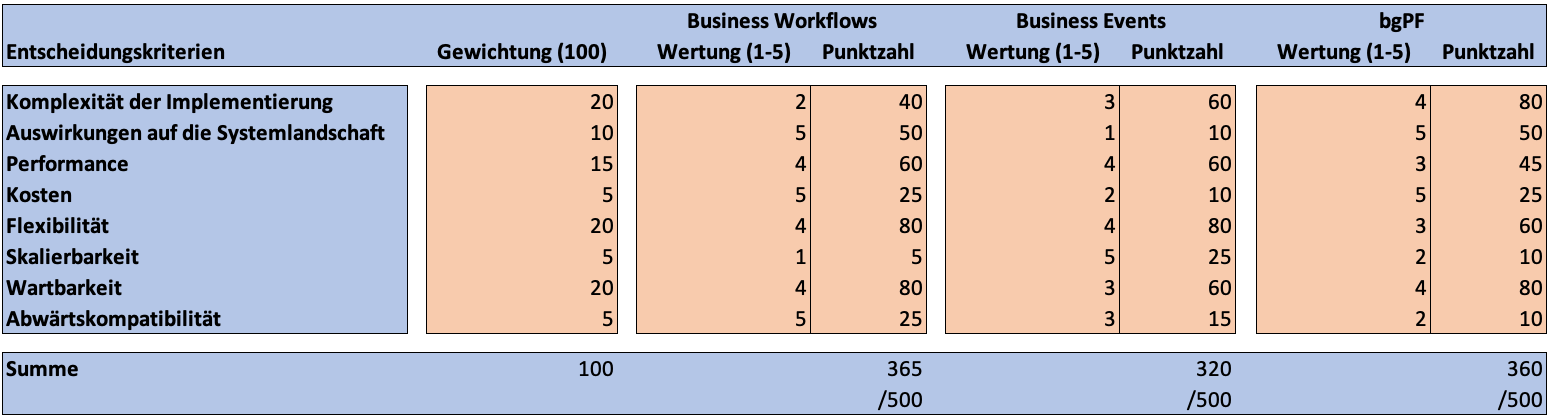
\includegraphics[height=4.3cm]{Bilder/Handlungsempfehlung_Entscheidungsmatrix.png}
 \caption[gewichtete Entscheidungsmatrix der drei Ansätze]{gewichtete Entscheidungsmatrix der drei Ansätze, eigene Darstellung}
 \label{fig:iso_norm}
\end{figure}

Die Gewichtungen der Kriterien wurden durch eine abteilungsinterne Befragung der für das Thema verantwortlichen Personen ermittelt. Die Wertungen der Technologien für die einzelnen Vergleichspunkte wurden aus dem Vergleich im vorhergehenden Kapitel bestimmt. Somit ergibt sich, dass die Technologie Business Workflows, die auch aktuell zum Lösen der Problemstellung im Betrieb zum Einsatz kommt tatsächlich, entgegen der anfänglichen Annahme die beste Variante ist, wenn auch der Unterschied zum bgPF nur sehr marginal ist. Da die Bewertungen relativ zueinander erfolgt sind und bei den beiden Technologien nur um 1\% abweichen, sollten diese als gleichwertig geeignet für die Lösung der Problemstellung betrachtet werden. Business Events würden sich zwar grundlegend auch für den Anwendungsfall eigenen, bieten aber insgesamt nicht so viele Vorteile wie die anderen beiden Ansätze. Allgemein hängt die Wahl von der spezifischen Gewichtung der einzelnen Kriterien ab. 

\section{Reflexion der Arbeit und Ausblick}


